% @author: Jan Svacina
% @author: Jonathan Simmons

\documentclass{article}


\usepackage{fullpage}
\usepackage{url}

\usepackage{amssymb}
\usepackage{amsmath}

%\let\emptyset\emptyset
%\let\emptyset\varnothing

\usepackage[letterspace=150]{microtype}

%\usepackage{enumitem}
%\usepackage{flexisym} % https://tex.stackexchange.com/questions/36655/prime-in-text-mode
%\usepackage{commath}
%\usepackage{graphicx}
%\graphicspath{ {./} }

\let\oldemptyset\emptyset
\let\emptyset\varnothing

    \usepackage{listings}
\usepackage{color}

%\definecolor{codegreen}{rgb}{0,0.6,0}
%\definecolor{codegray}{rgb}{0.5,0.5,0.5}
%\definecolor{codepurple}{rgb}{0.58,0,0.82}
%\definecolor{backcolour}{rgb}{0.95,0.95,0.92}
%
%\lstdefinestyle{mystyle}{
%backgroundcolor=\color{backcolour},
%commentstyle=\color{codegreen},
%keywordstyle=\color{magenta},
%numberstyle=\tiny\color{codegray},
%stringstyle=\color{codepurple},
%basicstyle=\footnotesize,
%breakatwhitespace=false,
%breaklines=true,
%captionpos=b,
%keepspaces=true,
%%numbers=left,
%numbersep=5pt,
%showspaces=false,
%showstringspaces=false,
%showtabs=false,
%tabsize=2,
%%basicstyle=\lage
%}
%
%\lstset{style=mystyle}

% tell Latex to use no paragraph indentation, but leave some space between
% paragraphs
\setlength{\parindent}{0in}
\setlength{\parskip}{0.1in}

\usepackage{hyperref}
\hypersetup{
colorlinks=true,
linkcolor=blue,
filecolor=magenta,
urlcolor=blue,
}
\urlstyle{same}

\lstset{
language=C,                % choose the language of the code
%numbers=left,                   % where to put the line-numbers
%stepnumber=1,                   % the step between two line-numbers.
numbersep=5pt,                  % how far the line-numbers are from the code
backgroundcolor=\color{white},  % choose the background color. You must add \usepackage{color}
showspaces=false,               % show spaces adding particular underscores
showstringspaces=false,         % underline spaces within strings
showtabs=false,                 % show tabs within strings adding particular underscores
tabsize=2,                      % sets default tabsize to 2 spaces
captionpos=b,                   % sets the caption-position to bottom
breaklines=true,                % sets automatic line breaking
breakatwhitespace=true,         % sets if automatic breaks should only happen at whitespace
title=\lstname,                 % show the filename of files included with \lstinputlisting;
}


\usepackage{graphicx}
\graphicspath{ {./images/} }
\usepackage[final]{pdfpages}
%\usepackage{fullpage}
%\usepackage{url}
%\usepackage{hyperref}
%\usepackage{amssymb}
%\usepackage{amsmath}
%\usepackage[letterspace=150]{microtype}
%\usepackage{enumitem}
%\usepackage{graphicx}
%\graphicspath{ {./images/} }
%
%\hypersetup{
%colorlinks=true,
%linkcolor=blue,
%filecolor=magenta,
%urlcolor=blue,
%}
%\urlstyle{same}
%% tell Latex to use no paragraph indentation, but leave some space between
%% paragraphs
%\setlength{\parindent}{0in}
%\setlength{\parskip}{0.1in}
%\usepackage[final]{pdfpages}


\title{Iteration II}
\date{10/24/19}
\author{Jonathan Simmons, Jan Svacina}

\begin{document}

    \maketitle

    \lstinputlisting[mathescape=true, escapechar=\%, language=python, caption=generate conditions,
    captionpos=b]{snippets/gen-cond.py}

    \lstinputlisting[mathescape=true, escapechar=\%, language=python, caption=conditionals.py,
    captionpos=b]{snippets/conditionals.py}

    \lstinputlisting[mathescape=true, escapechar=\%, language=python, caption=creating-training.py,
    captionpos=b]{snippets/creating-training.py}

    \lstinputlisting[mathescape=true, escapechar=\%, language=python, caption=imports.py,
    captionpos=b]{snippets/imports.py}

    \lstinputlisting[mathescape=true, escapechar=\%, language=python, caption=predicate.py,
    captionpos=b]{snippets/predicate.py}

    \lstinputlisting[mathescape=true, escapechar=\%, language=python, caption=rading.py,
    captionpos=b]{snippets/reading.py}

    \lstinputlisting[mathescape=true, escapechar=\%, language=python, caption=conditionals.py,
    captionpos=b]{snippets/running-model.py}

    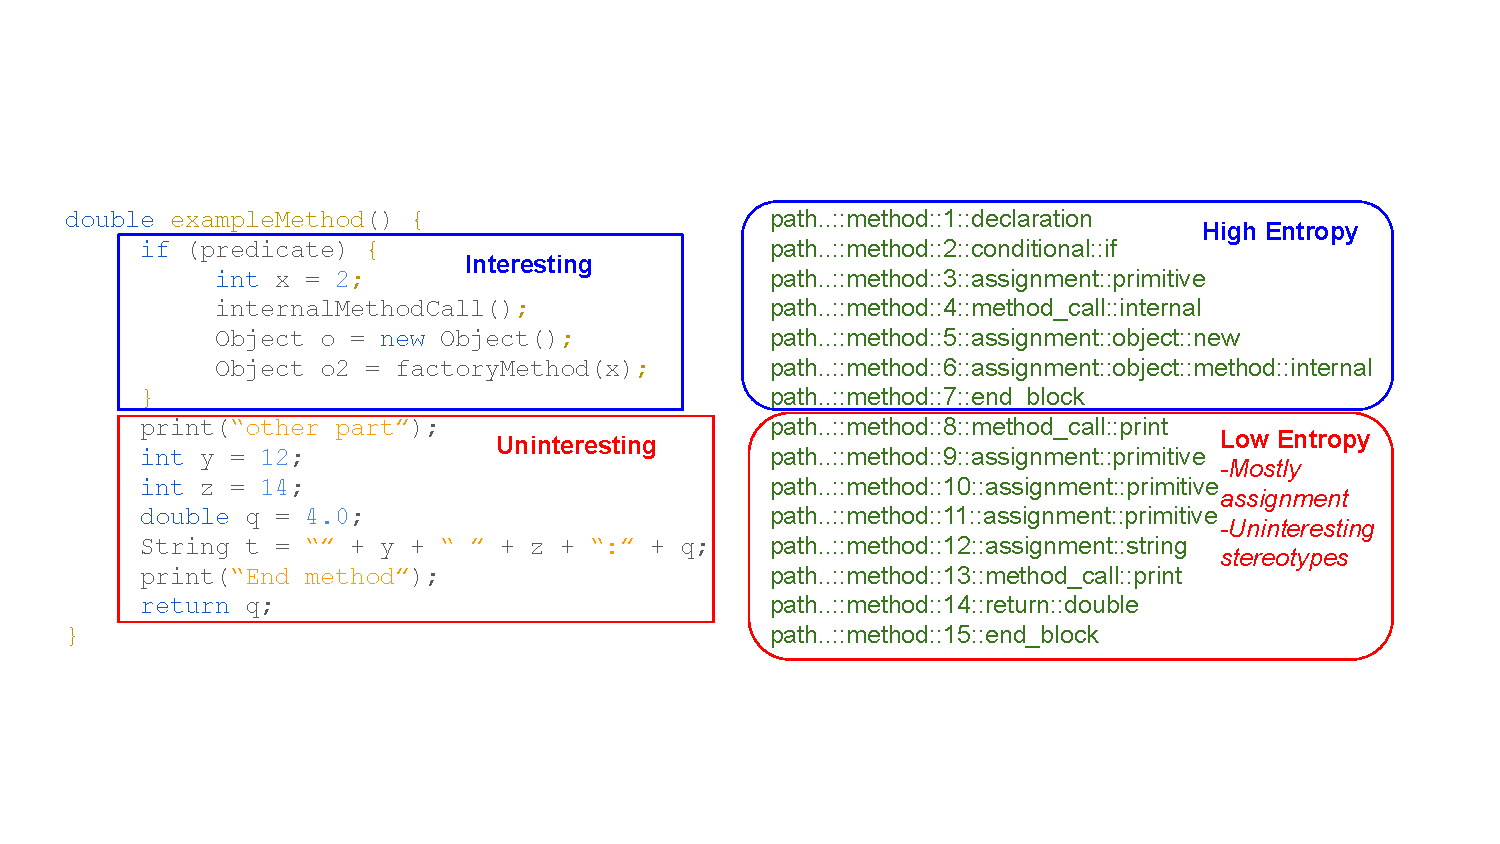
\includepdf[pages=-,pagecommand={},width=\textwidth]{images/01.pdf}

    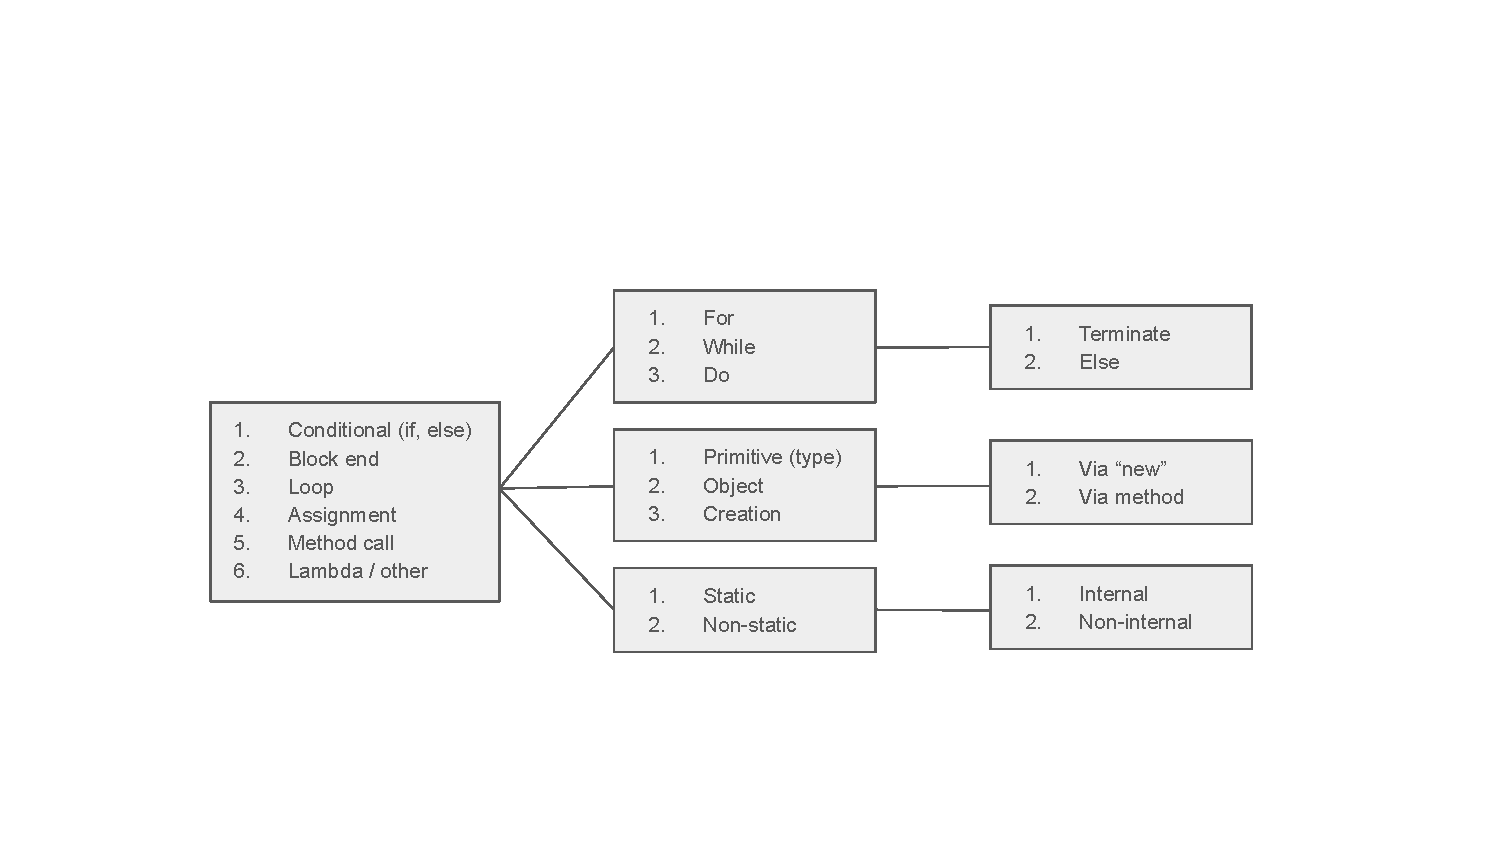
\includepdf[pages=-,pagecommand={},width=\textwidth]{images/02.pdf}

    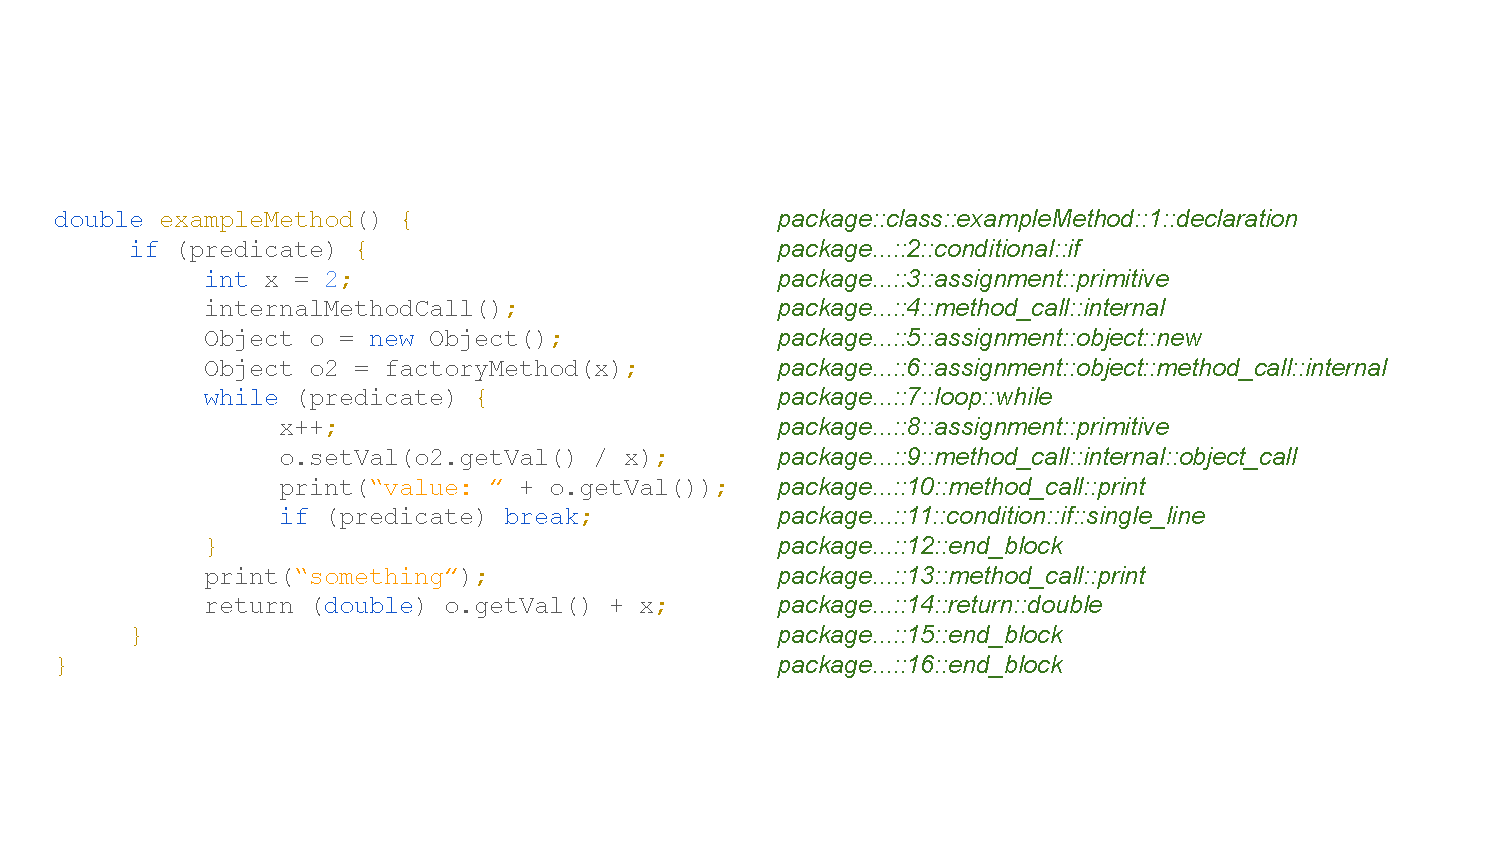
\includepdf[pages=-,pagecommand={},width=\textwidth]{images/03.pdf}


    \section*{Summary}


    \subsection*{Jonathan Simmons}

    \begin{center}
        \begin{tabular}{||c c ||}
            \hline
            Number of tasks: &  \\
            \hline
            Number of commits: &  \\
            \hline
            Number of hours: &  \\
            \hline
        \end{tabular}
    \end{center}

    \subsection*{Jan Svacina}

    \begin{center}
        \begin{tabular}{||c c ||}
            \hline
            Number of tasks: &  \\
            \hline
            Number of commits: &  \\
            \hline
            Number of hours: &  \\
            \hline
        \end{tabular}
    \end{center}




\end{document}
